\section{Kalibrierung des Röntgendetektors}

Der Versuch wird wie in der Vorbereitung beschrieben durchgeführt.
Dabei konnte kein Nutzen durch die Verwendung einer höheren Verstärkungsstufe beobachtet werden, die K$_\alpha$ und K$_\beta$-Linien der Standardproben ließen sich auch bei V = 4 nicht klar voneinander unterscheiden. Die Kalibrierung wird daher auch nur anhand der K$_\alpha$-Linien durchgeführt.\\
Einzige Ausnahme bildet Silber, bei welchem im Röntgenspektrum zwei klar erkennbare Peaks vorhanden waren. Diese lagen allerdings in einem so hohen Energiebereich, dass sie mit einer Verstärkung von V = 4 nicht mehr auf der Skala gewesen wären.\\
Bei Blei und Wolfram handelt es sich außerdem um die L$_\alpha$ und L$_\beta$-Linien, da die K$_\alpha$-Linie deutlich höher als die maximal erreichbaren 35\;keV liegt.\\
Die gefitteten Peaks der einzelnen Proben befinden sich in Tabelle \ref{tab:a1_peaks}.

\xtable{htb}{a1_peaks}{Messwerte der Fits unterschiedlicher Röntgenspektren}{(Aufg. 1)}

Die Gleichung der mit Hilfe von QtiPlot an die Messwerte f\"ur V = 2 gefitteten Gerade (s. Abb. \ref{fig:a1_fit}) inkl. statistischer Fehler sieht folgendermaßen aus:
\begin{equation}
	E_2(K) = (0,00807\pm 0,00002)K\cdot\si{\kilo\electronvolt} + (1,40\pm 0,04)\cdot\si{\kilo\electronvolt}
\end{equation}

\begin{figure}[h]
	\centering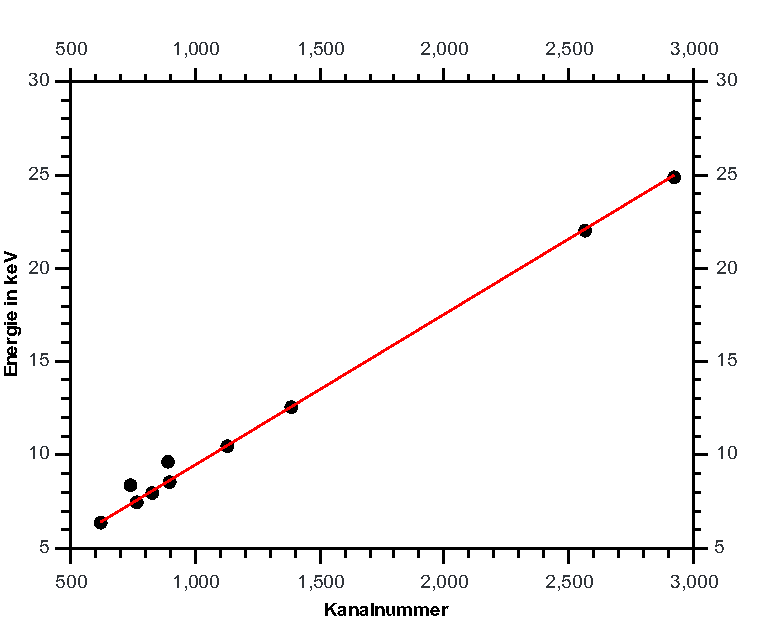
\includegraphics[width=0.8\textwidth]{fig/a1_fit}
	\caption{Skalierungsgerade zur Eichung des Röntgendetektors mit V = 2.}
	\label{fig:a1_fit}
\end{figure}

Es ist zu erkennen, dass die Messwerte der Röntgenstrahlung ohne Materialprobe als einzige von der Geraden abweichen und die Regression bei niedrigeren Kanalnummern nach oben ziehen. Dies liegt daran, dass die Zählrate in diesem Versuchsteil zu hoch war und der VKA somit überfordert wurde. Die Messwerte sind daher in Abb. \ref{fig:a1_fit} aufgeführt, wurden aber für die lineare Regression nicht verwendet.

Da zur Bestimmung der Energieauflösung die Verstärkungsstufe 4 benutzt wurde, wird auch zu diesen Messwerten eine Kalibrierung durchgeführt.
\begin{equation}
	E_4(K) = (0,00406\pm 0,00001)K\cdot\si{\kilo\electronvolt} + (1,366\pm 0,016)\cdot\si{\kilo\electronvolt}
\end{equation} 

\begin{figure}[h]
	\centering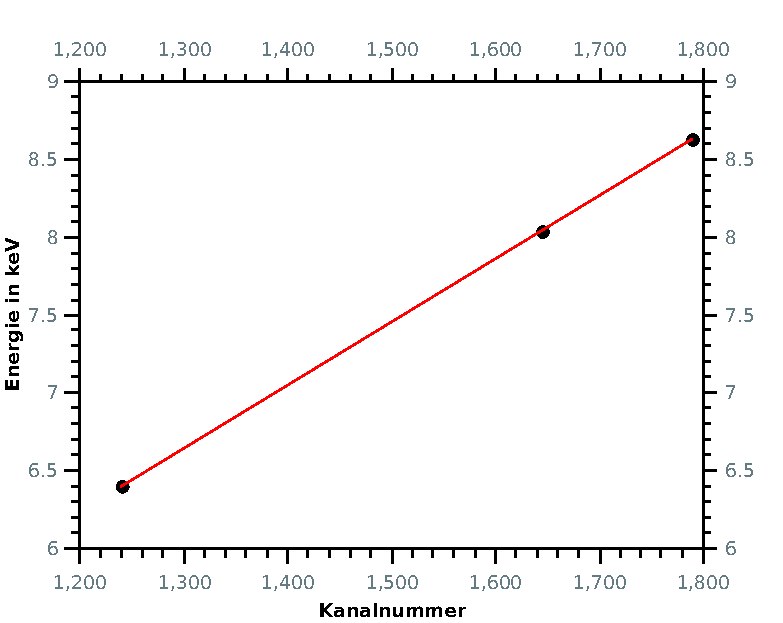
\includegraphics[width=0.8\textwidth]{fig/a1_fit_4}
	\caption{Skalierungsgerade zur Eichung des Röntgendetektors mit V = 4.}
	\label{fig:a1_fit_4}
\end{figure}

\section{Bestimmung der Energieauflösung des RED}
Der Versuch wurde wie in der Vorbereitung beschrieben durchgeführt.
Die gemessenen und aus den Messwerten errechneten Werte befinden sich in Tabelle \ref{tab:a2}.\\

\xtable{htb}{a2}{Messwerte zur Bestimmung der Energieauflösung}{(Aufg. 2)}

In Abbildung \ref{fig:a2_energie_breite} sind die gemessene Energie der K$_\alpha$ Linie von Zink und der Halbwertsbreite dieser Linie gegen die Zählrate aufgetragen.

\begin{figure}[h]
	\centering
	\subfigure[]{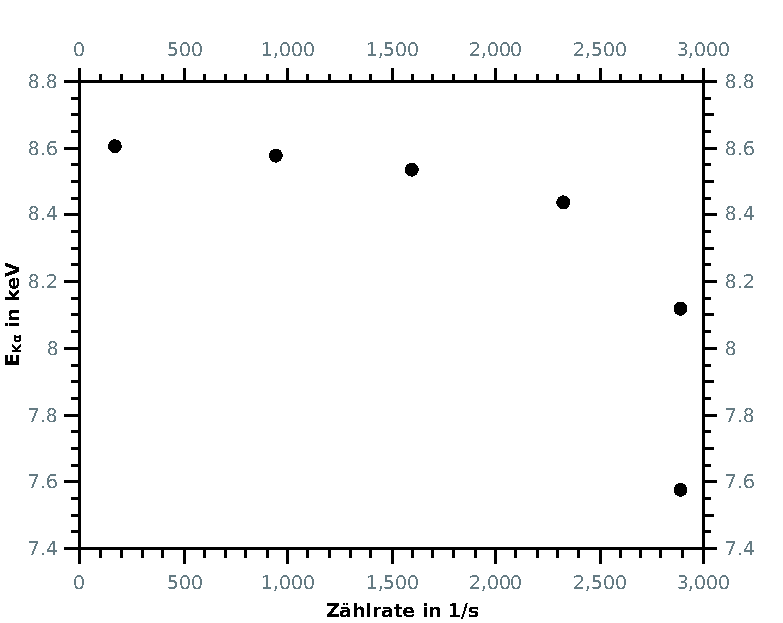
\includegraphics[width=0.49\textwidth]{fig/a2_energie}}
	\subfigure[]{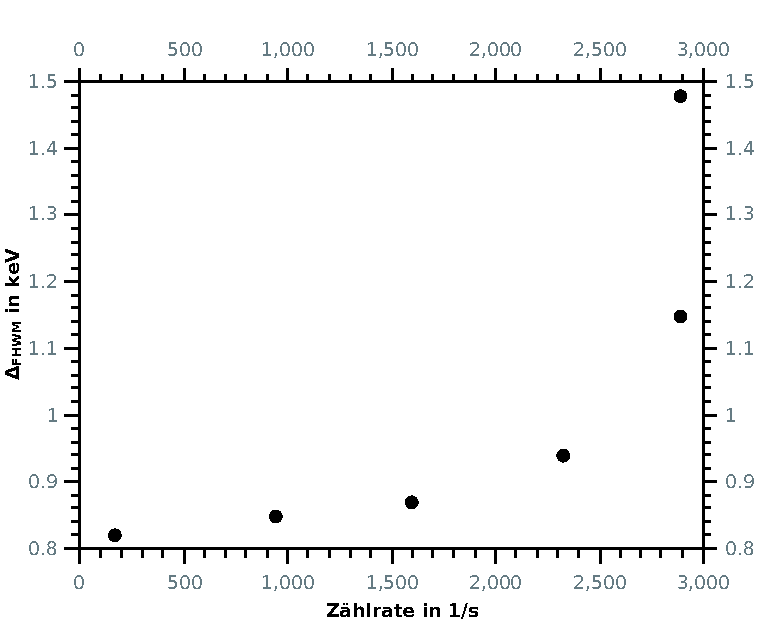
\includegraphics[width=0.49\textwidth]{fig/a2_breite}}
	\caption{\textbf{a)} Energie der K$_\alpha$-Linie gegen die Zählrate aufgetragen, \textbf{b)} Halbwertsbreite der K$_\alpha$-Linie.}
	\label{fig:a2_energie_breite}
\end{figure}

Es ist klar ein exponentielles Wachstum bei der Halbwertsbreite, bzw. ein exponentieller Zerfall bei der gemessenen Energie in der Abhängigkeit von der Zählrate zu erkennen. Bis zu einer Zählrate von 1500\;$\frac{1}{s}$ ist die gemessene Energie und Halbwertsbreite näherungsweise konstant, es empfiehlt sich also bei weiteren Messungen unterhalb dieses Wertes zu bleiben.\\
Der letzte Wert, der bei einem Emissionsstrom von 1\;mA gemessen wurde,liegt auf der gleichen Zählrate wie der Wert für 0,5\;mA. Das liegt vermutlich daran, dass der VKA nur maximal 2885 Ereignisse pro Sekunde aufzeichnen kann und somit beide Werte über dieser Schwelle liegen.\\

\section{Qualitative Röntgenfluoreszensanalyse}

Die Daten wurden nicht neu gemessen, sondern nach Absprache mit dem Betreuer aus den Messungen des ersten Versuchs übernommen.
\begin{figure}[h]
	\centering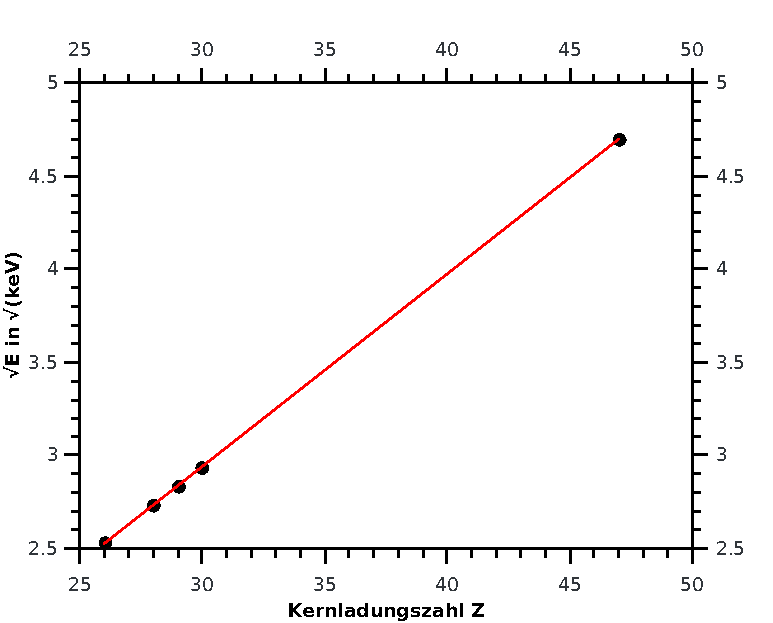
\includegraphics[width=0.8\textwidth]{fig/a3_fit}
	\caption{Lineare Regression zur Bestimmung der Rydberg- und Moseleykonstante.}
	\label{fig:a3_fit}
\end{figure}
Die Regression $m\cdot Z + C$ in Abb. \ref{fig:a3_fit} wurde mit Qtiplot durchgeführt und hat folgende Werte:
\begin{align}
	m &= 0,10342\pm 0,00015\\
	c &= -0,162\pm 0,005
\end{align}
Mit Gaußscher Fehlerfortpflanzung und Gleichung \ref{eq:rhydberg} lässt sich die Rydbergkonstante bestimmen:
\begin{equation}
	R_{\infty} = (1,150\cdot 10^{7}\pm 3,3\cdot 10^{4})\;\si{\metre}^{-1}
\end{equation}

Die Abschirmungskonstante $\sigma_{2,1}$ kann mithilfe von Gleichung \ref{eq:abschirm} bestimmt werden:
\begin{equation}
	\sigma_{2,1} = 1,604\pm 0,002
\end{equation}
Da die K$_\beta$-Linien nicht klar erkennbar waren, da die Auflösung des Röntgendetektors zu schlecht ist, lässt sich keine Aussage zur Abschirmkonstante $\sigma_{3,1}$ treffen.\\
Die Abweichung der gemessenen Rydbergkonstante zum Literaturwert beträgt nur 4,7\;\%.

\section{Bestimmung der Schichtdicke dünner Folien}

In diesem Versuch wird die Schichtdicke von Aluminiumfolie mit Hilfe des RED gemessen. Dazu wird eine Eisenprobe verwendet, mit Alufolie abgedeckt, und die Abschwächung der Intensität der charakteristischen Linien in Abhängigkeit der Anzahl der Folien gemessen.
Wie in der Vorbereitung beschrieben gilt für die Intensität
\begin{equation}
 I = I_{0}\exp\left(\mu\rho x\right),
\end{equation}
mit der Anfangsintensität $I_{0}$, der Dichte $\rho$ und dem Massenabsorptionskoeffizienten $\mu$.
Daraus ergibt sich
\begin{equation}
 \ln\left(\frac{I}{I_{0}}\right) = \mu\rho x.
\end{equation}
Für die Strecke $x$ gilt
\begin{equation}
 x = 2\sqrt{2}dn,
\end{equation}
mit der Schichtdicke $d$ und der Anzahl der Schichten $n$. Der Vorfaktor kommt daher, dass die Probe in einem Winkel von $\alpha=\SI{45}{\degree}$ zur Strahlrichtung steht (s. Abb. \ref{fig:41}) und der Strahl die Probe zweimal durchquert. 
Insgesamt ergibt sich also
\begin{equation}
 \ln\left(\frac{I}{I_{0}}\right) = 2\sqrt{2}\mu\rho dn. 
\end{equation}
Die Schichtdicke kann nun aus einer linearen Regression der Form $\ln\left(\frac{I}{I_{0}}\right)(n) = an+b$ bestimmt werden.

\xtable{tb}{a4_tab}{Gemessene Peaks in Abhängigkeit der Anzahl der Schichten}{(Aufg. 4)}

Die Messwerte sind in Tab. \ref{tab:a4_tab} aufgeführt.
Die lineare Regression wird mit ``QtiPlot'' durchgeführt (s. Abb. \ref{fig:42}) und ergibt
\begin{align}
 a &= -0,54 \pm 0,04, \\
 b &= -0,12 \pm 0,17.
\end{align}
Da für Aluminium gilt $\rho=\SI{2,7}{\gram\per\centi\metre\cubed}$ und $\mu=\SI{92,8}{\centi\metre\squared\per\gram}$ \cite{litmap}, ergibt sich für die Schichtdicke
\begin{equation}
 d = -\frac{a}{2\sqrt{2}\mu\rho} = \SI{7,6\pm0,6}{\micro\metre}.
\end{equation}
In der Literatur findet sich für die Dicke von Aluminiumfolie $d\approx\SI{10}{\micro\metre}$ bis $\SI{15}{\micro\metre}$ \cite{wiki}. Dies liegt in der gleichen Größenordnung wie unser Ergebnis.
%
\begin{figure}[tb]
 \centering
 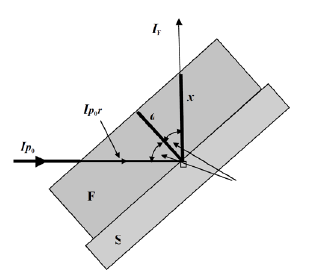
\includegraphics[scale=0.6]{./fig/a4_bild.png}
 \caption{Schematische Skizze des Versuchsaufbaus (Quelle: \cite{litmap})}
 \label{fig:41}
\end{figure}

\begin{figure}[tb]
 \centering
 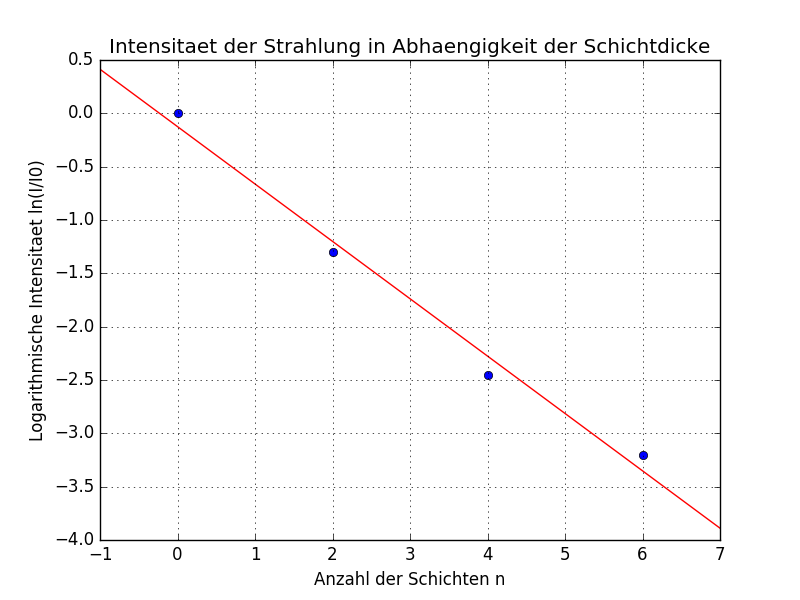
\includegraphics[scale=0.6]{./fig/a4_plot.png}
 \caption{Intensität der Röntgenstrahlung in Anhängigkeit der Schichtdicke}
 \label{fig:42}
\end{figure}

\section{Qualitative Röntgenfluoreszenzanalyse an Legierungen}

In diesem Versuch wird die Zusammensetzung von Legierungen bestimmt. Dazu werden die charakteristischen Linien der Legierung bestimmt und mit bekannten Linien verglichen. Für die Konzentration $C$ gilt
\begin{equation}
 C = \frac{I}{I_{el}},
\end{equation}
wobei $I_{el}$ die Intensität der Linie beim reinen Element ist. Es werden die Probe A (Lötzinn), Probe D (Konstantan), Probe E (Hartmetallfräser) und eine 5-Cent-Münze untersucht.

\subsection{Probe A (Lötzinn)}

Bei der Probe A handelt es sich um ein schneckenförmig zusammengerolltes Stück Draht aus Lötzinn. Die gemessenen Peaks sind in Tab. \ref{tab:a6_probe_a} aufgeführt. Die Peaks bei $a=263$ und $a=3354$ lassen sich nicht zuordnen, da für diese Kanalnummern keine charakteristischen Linien gemessen wurden.
Bei den restlichen Linien handelt es sich vermutlich um Kupfer und die zwei Silber-Linien. Für Kupfer ergibt sich eine Konzentration von
\begin{equation}
 C = 2,9\%,
\end{equation}
und für Silber
\begin{align}
 C_{1} &= 10,4\%, \\
 C_{2} &= 150,3\%.
\end{align}
Vermutlich handelt es sich beim zweiten Messwert um einen Messfehler, möglicherweise wurde die K$_{\beta1}$-Linie von Silber von einer anderen Linie überlagert. Daher wird nur der Wert der K$_{\alpha}$-Linie verwendet.
Um die Zusammensetzung zu erhalten, werden die Werte noch auf $100\%$ skaliert. Vermutlich wurde nicht alle Röntgenstrahlung zur Erzeugung charakteristischer Linien verwendet, da die Probe Zwischenräume besaß.
Es ergibt sich
\begin{align}
 C_{\textrm{Cu}} &= 22\%, \\
 C_{\textrm{Ag}} &= 78\%.
\end{align}

Laut \cite{wiki_lot} befindet sich in Lötzinn hauptsächlich Blei, Zinn, Zink, Silber und Kupfer. Es ist also zu vermuten, dass die Hauptkomponenten des Lötzinns und deren Anteil einigermaßen genau bestimmt wurde.

\xtable{htb}{a6_probe_a}{Gemessene Peaks für Probe A}{(Aufg. 6)}

\subsection{Probe D (Konstantan)}

Bei der Konstantan-Probe war nur eine Linie sichtbar. Diese besaß die folgenden Parameter:
\begin{align}
 a &= 611, \\
 c &= 14805. 
\end{align}
Somit handelt es sich vermutlich um die Linie von Eisen. Die Konzentration beträgt
\begin{equation}
 C = 37,3\%. 
\end{equation}
Der Grund dafür, dass $C<100\%$ ist vermutlich, dass der Strahl auch neben der Probe auftraf, und somit nicht die gesamte Intensität verwendet wurde. Laut \cite{wiki_konst} besteht Konstantan zu $55\%$ aus Kupfer, zu $44\%$ aus Nickel und zu $1\%$ aus Mangan.
Der Grund für die Abweichung könnte darin bestehen, dass der Probenhalter Eisen enthielt.

\subsection{Probe E (Hartmetallfräser)}

Die gemessenen Peaks für Probe E sind in Tab. \ref{tab:a6_probe_e} aufgeführt. Bei der Linie bei $a=685$ handelt es sich vermutlich um Eisen. Dessen Konzentration ergibt sich zu
\begin{equation}
 C_{\textrm{Fe}} = 7,3\%.
\end{equation}
Die restlichen Linien sind schwieriger zuzuordnen. Die Linie bei $a=858$ deutet auf Zink hin, vor allem da sich auch bei $1024$ eine Linie befindet, was zur K$_{\beta}$-Linie von Zink passen würde. Die Verhältnisse stimmen jedoch nicht überein. 
Der Grund dafür ist möglicherweise, dass die Linie von der L$_{\alpha}$-Linie von Blei überlagert wird. Die Linie bei $1226$ könnte zur L$_{\beta}$-Linie von Blei passen. Werden die Linien Zn K$_{\alpha}$ und Pb L$_{\beta}$ zur Bestimmung der Konzentration verwendet, so ergibt sich
\begin{align}
 C_{\textrm{Zn}} &= 13,8\%, \\
 C_{\textrm{Pb}} &= 11,7\%.
\end{align}
Werden die Konzentrationen auf $100\%$ skaliert, so ergibt sich
\begin{align}
 C_{\textrm{Fe}} &= 22\%, \\
 C_{\textrm{Zn}} &= 42\%, \\
 C_{\textrm{Pb}} &= 36\%.
\end{align}
Tatsächlich besteht der Fräser aus Wolframcarbid. Vermutlich wurden die Peaks in der Vergleichsmessung in Aufgabe 1 dem falschen Kanal zudeordnet, da die Zählrate zu hoch war. 

\xtable{htb}{a6_probe_e}{Gemessene Peaks für Probe E}{(Aufg. 6)}

\subsection{5-Cent-Münze}

Bei der 5-Cent-Münze war nur eine Linie sichtbar. Diese besaß die Parameter
\begin{align}
 a &= 819, \\
 c &= 515176. \\
\end{align}
Es handelt sich dabei vermutlich um Kupfer. Die Konzentration beträgt
\begin{equation}
 C = 98,4\%.
\end{equation}
Laut \cite{wiki_5ct} bestehen 5-Cent-Münzen aus Eisen mit Kupferummantelung. Vermutlich konnte die Röntgenstrahlung nicht bis zum Eisenkern vordringen, weshalb nur das Kupfer gemessen wurde.
